\chapter{失智症之認知功能評估}
\label{chapter:intro}
\section{簡易智能評估(Mini-Mental State Examination,MMSE)}
為臨床上最廣泛應用評估老年人認知狀態之工具,共分為定向感、記錄能力、注意力和計算力、回憶能力、抽象概念和語言能力來評估,滿分是三十分,答對一項給一分,若低於二十三分表度知能損傷,低於十六分表重度認知功能損傷。


是Folstein等人1975年所提出,2001年3月MMSE版權已轉為PAR, Inc.所有,任何臨床上使用、論文發表及研究使用需至PAR,Inc.網站申請版權使用。

認知評估項目:
\begin{enumerate}
	\item
    定向感(時間地點)
	\item
	注意力與算術能力
	\item
    立即記憶與短期記憶
	\item
	語言能力:讀、寫、命名、理解與操作
	\item
    視覺空間能力
\end{enumerate}


\section{簡易心智狀態問卷(Short Portable Mental State Questionnaire,SPMSQ)}
可以用來快速檢測家中的長輩是否有失智的風險
\begin{figure}[H]
	\centerline{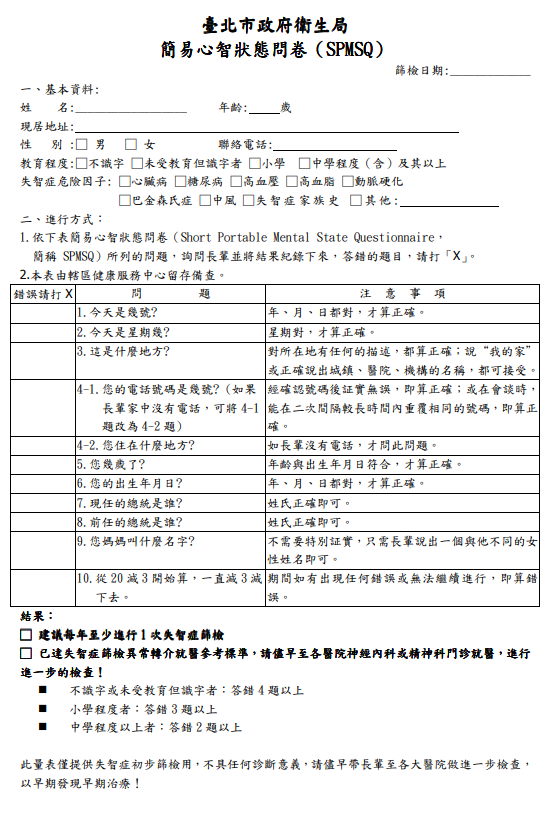
\includegraphics[height=18cm]{pic/SPMSQ.PNG}}
	\caption{C簡易心智狀態問卷(SPMSQ)\\來源:臺北市政府衛生局}
	
	\label{fig:SPMSQ}
\end{figure}

\label{sec:background}
\section{臨床失智評估表 ( Clinical Dementia Rating,CDR)}

具有輕微認知症狀(例如記憶力下降)的患者是否患有前期或臨床前阿茲海默氏病(Alzheimer disease,AD)並在不久的將來發展為 AD 癡呆仍然是臨床醫生面臨的挑戰。這項任務對於正確和早期的 AD 診斷、開始對AD症治療、規劃未來以及希望很快開始改善疾病的治療都至關重要。

美國華盛頓大學的Hughes等人提出,用來評估阿茲海默 症患者日常生活及認知功能作整體性評估的量表。

\begin{figure}[H]
	\centerline{\includegraphics[height=20cm]{pic/CDR.PNG}}
	\caption{CDR 臨床失智評分量表\\來源:衛生福利部,失智症診療手冊}
	
	\label{fig:CDR}
\end{figure}




\section{神經心理衡鑑(CASI)}
認知功能障礙篩檢量表 (CASI):包含25題,滿分為一百分,經由固定的換算方式可以把它化成9個認知功能的細項,分別是長期記憶,短期記憶、時間空間定向感、注意力、心智操作和集中力 、思考流暢度,語言及基本認知功能、抽象思考能力及判斷力和手眼協調構圖能力。


%\section{附錄:MMSE和CDR}

%\includepdf[pages={1,2,3,4,5,6,7,8,9,10,11}]{MMSE.pdf}

%\includepdf[pages={1,2,3,4,5,6,7,8}]{CDR.pdf}

